\section{External Interface Requirements}

\subsection{User Interfaces}

The system will provide a web-based user interface that caters to all user groups—students, companies, and universities. Each user group will have distinct interfaces designed to facilitate their respective roles. The interface must be intuitive, and supporting a seamless user experience for desktop devices. \\ \\
\vspace{5mm}
\textbf{For Students:}
\begin{itemize}
    \item \textbf{Recommendation Page}: Upon logging in, students will have access to a personalized page displaying recommended internships and company invites.
    \item \textbf{Profile Management}: The user interface will allow students to edit their profiles, including personal details, interests, and skills. It must support file uploads for CVs in common formats (PDF, DOCX).
    \item \textbf{Internships page}: Students will have access to an internship page with a  search tool to filter internships by criteria such as name or localization.
    \item \textbf{Application Process}: A step-by-step guided process will follow students through the application process. The interface will show application deadlines, company requirements, and allow students to track their progress (e.g., application submitted, online assessment, etc.).
\end{itemize}
\vspace{5mm}
\textbf{For Companies:}
\begin{itemize}
    \item \textbf{Internship Posting}: Companies will have a separate interface to create detailed internship postings. The interface will include fields for defining the role, required skills, compensation details, deadlines, and online assessment questions.
    \item \textbf{Candidate Review}: Companies will have a space that lists for each internship the students who have applied, including a summary of the students' profiles and CVs.
    \item \textbf{Recommendation Feed}: The interface will provide companies with a list of recommended candidates based on internship requirements, allowing them to invite those promising students to apply.
\end{itemize}
\vspace{5mm}
\textbf{For Universities:}
\begin{itemize}
    \item \textbf{Monitoring Dashboard}: Universities will have access to a dashboard for overseeing the overall situation of internships, addressing complaints, and tracking student-company interactions. The dashboard will include a summary view of ongoing internships and flagged issues.
    \item \textbf{Complaint Management}: Universities will have a space dedicated to the complaints management. Administrators can log, track, and update complaint statuses through the interface, ensuring a transparent process for all parties involved.
\end{itemize}

\subsection{Hardware Interfaces}

The platform does not require specialized hardware; users only need a computer with an Internet connection to interact with the platform's servers.

\subsection{Software Interfaces}

The Students\&Companies (S\&C) platform interacts with various external software systems and tools to ensure its functionalities. The key software interfaces are as follows:

\begin{itemize}
    \item \textbf{Database Interface:}
    \begin{itemize}
        \item The system interacts with a relational database management system (e.g., PostgreSQL, MySQL) to store and retrieve user data, internship details, feedback, and recommendations.
        \item The platform must ensure consistent data transactions (CRUD operations) with integrity and security.
    \end{itemize}

    \item \textbf{Email Service Interface:}
    \begin{itemize}
        \item The platform integrates with an external email service (e.g., SMTP server or third-party services like SendGrid) to send notifications for registration confirmation, interview schedules, internship updates, and feedback submissions.
    \end{itemize}

    \item \textbf{Web Browser Compatibility:}
    \begin{itemize}
        \item The system interfaces with modern web browsers (e.g., Chrome, Firefox, Safari) to ensure usability and consistent rendering of the web-based user interface.
    \end{itemize}

    \item \textbf{File Upload and Validation Interface:}
    \begin{itemize}
        \item The system supports file uploads (e.g., PDF for CVs) and integrates with tools to validate file format, size, and content security.
    \end{itemize}
\end{itemize}


\subsection{Communication Interfaces}

The platform will use HTTPS for all communications to ensure secure data transmission between users and the system.\\ \\
Email notifications will be sent using industry-standard email protocols (SMTP) with TLS encryption to ensure secure communication. \\ \\
All this is done to ensure that users are promptly notified of important actions (e.g., internship recommendations) in real-time.
\newpage

\section{Functional Requirements}
\subsection{Use case diagrams}
\begin{figure}[ht!]
    \centering
    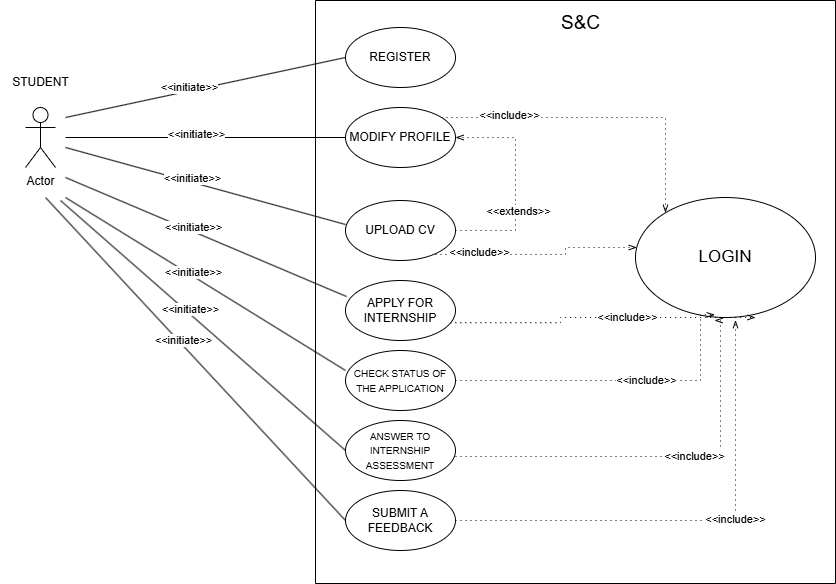
\includegraphics[scale=0.40]{Images/ImagesRASD/ScenariosStateDiagram-UseCaseDiagrams_Student.drawio.png}
    \caption{Student use case diagram}
\end{figure}

\begin{figure}[ht!]
    \centering
    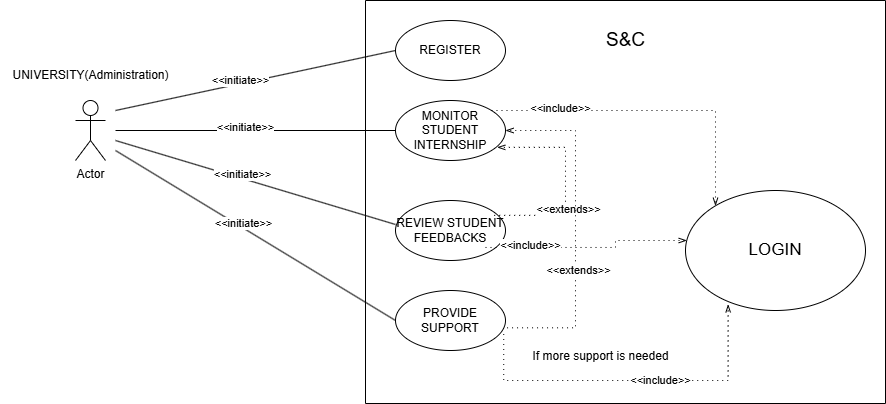
\includegraphics[scale=0.40]{Images/ImagesRASD/ScenariosStateDiagram-UseCaseDiagram_Universities.drawio.png}
    \caption{University use case diagram}

\end{figure}

\begin{figure}[ht!]
    \centering
    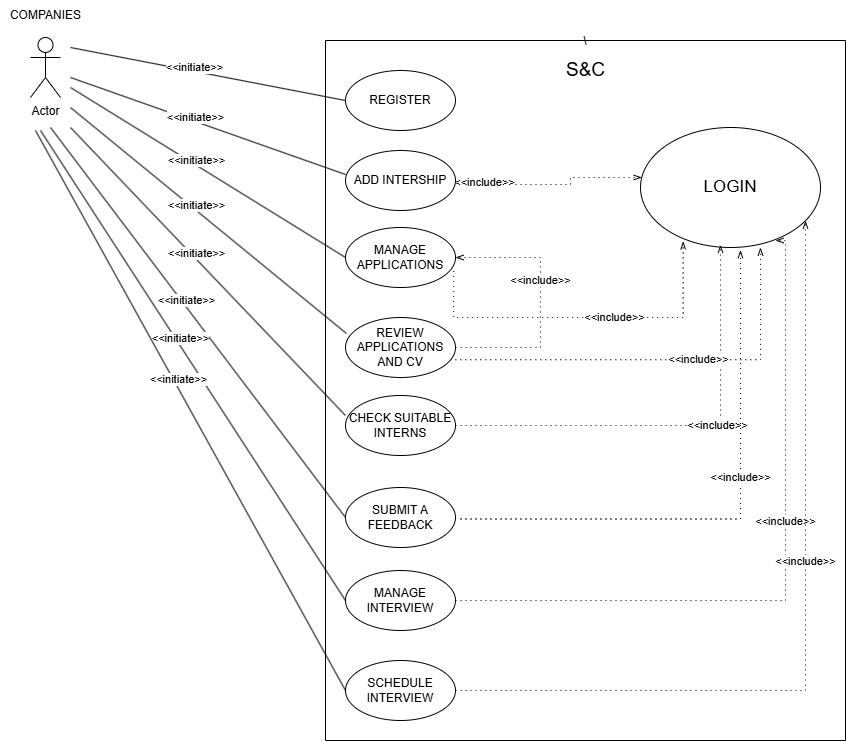
\includegraphics[scale=0.40]{Images/ImagesRASD/ScenariosStateDiagram-UseCaseDiagram_Companies.drawio.png}
    \caption{Company use case diagram}

\end{figure}

\clearpage

\subsection{Use cases}
\textbf{1) User registration use case}\\
\begin{table}[h!]
    \centering
    \begin{tabular}{lp{10cm}}
        \textbf{Actor} & User \\ \hline
        \textbf{Entry conditions} & The user is on the registration page of the S\&C platform and is ready to provide registration data. \\ \hline
        \textbf{Event Flow} &
        1. The user provides registration data \\
        & 2. S\&C platform validates the given data. \\
        & 3a. If the email is already registered, the platform returns an error: "Email already registered". \\
        & 3b. If the data is valid, the registration is successful. \\
        & 4. The user receives the confirmation email. \\
        & 5a. she user clicks the confirmation link within 24 hours. \\
        & 5b. If not, the user can request to resend the confirmation email. \\
        \hline
        \textbf{Exit condition} & The user registration process is successfully completed. The user might have confirmed his email. \\ \hline
        \textbf{Exceptions} &
        3.a. The email is already registered. \\
    \end{tabular}
    \caption{User registration use case}
    \label{tab:user_registration}
\end{table}

\begin{center}
    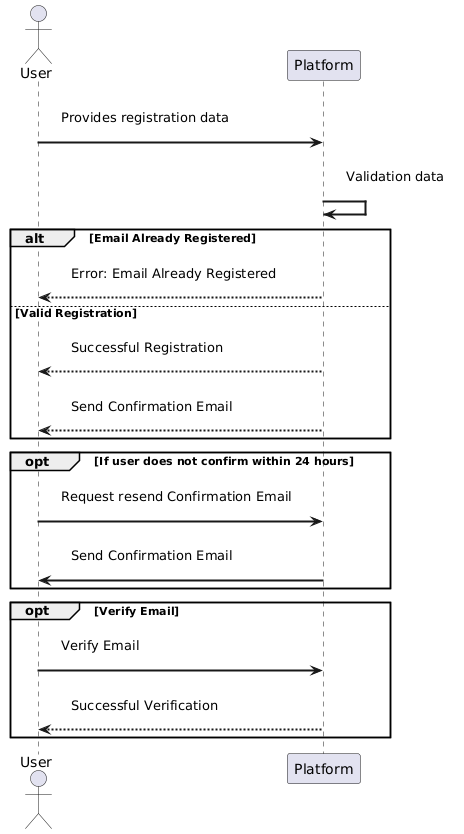
\includegraphics[scale = 0.8]{Images/ImagesRASD/user_registration.png}
\end{center}
\newpage
\textbf{2) User Login}\\

\begin{table}[h!]
    \centering
    \begin{tabular}{lp{10cm}}
        \textbf{Actor} & User \\ \hline
        \textbf{Entry conditions} & The user is on the login page of the S\&C platform, ready to enter credentials. \\ \hline
        \textbf{Event Flow} &
        1. The user provides their login credentials \\
        & 2. The S\&C platform validates the credentials. \\
        & 3a. If the credentials are valid, the platform successfully logs in the user. \\
        & 3b. If the credentials are invalid, the platform returns an error: "Invalid email or password" \\
        \hline
        \textbf{Exit condition} & The user is logged into the platform if the credentials are valid. \\ \hline
        \textbf{Exceptions} &
        3. Invalid email or password provided. \\
    \end{tabular}
    \caption{User login use case}
    \label{tab:user_login}
\end{table}


\begin{center}
    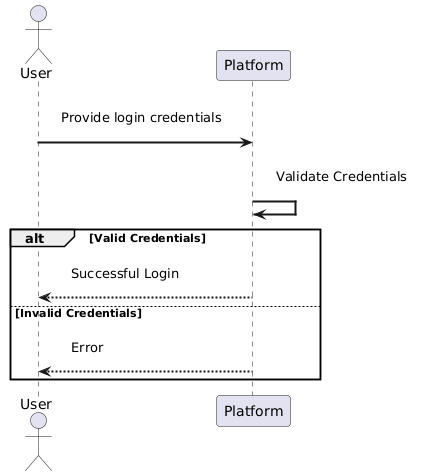
\includegraphics[scale = 1]{Images/ImagesRASD/user_login.png}
\end{center}

\newpage
\textbf{3) Internship post creation use case}\\

\begin{table}[h!]
    \centering
    \begin{tabular}{lp{10cm}}
        \textbf{Actor} & Company \\ \hline
        \textbf{Entry conditions} & The company is correctly logged on the platform and it is ready to create a new internship post. \\ \hline
        \textbf{Event Flow} &
        1. The company fills out the internship information form. \\
        & 2. The S\&C platform validates the internship data. \\
        & 3a. If the data is valid, the platform creates the new internship post and confirms success to the company. \\
        & 3b. If the data is invalid, the platform returns an error: "Error in internship data, please correct the form." \\
        & 4. The platform performs matching to find relevant students for the internship post. \\
        & 5. For each student that matches, the platform sends an internship post notification. \\
        \hline
        \textbf{Exit condition} & A new internship post is successfully created on the platform, and matching notifications are sent to relevant students. \\ \hline
        \textbf{Exceptions} &
        3. Invalid internship data: The company must correct and resubmit the form until valid data is provided. \\
    \end{tabular}
    \caption{Internship post creation use case}
    \label{tab:internship_post_creation}
\end{table}



\begin{center}
    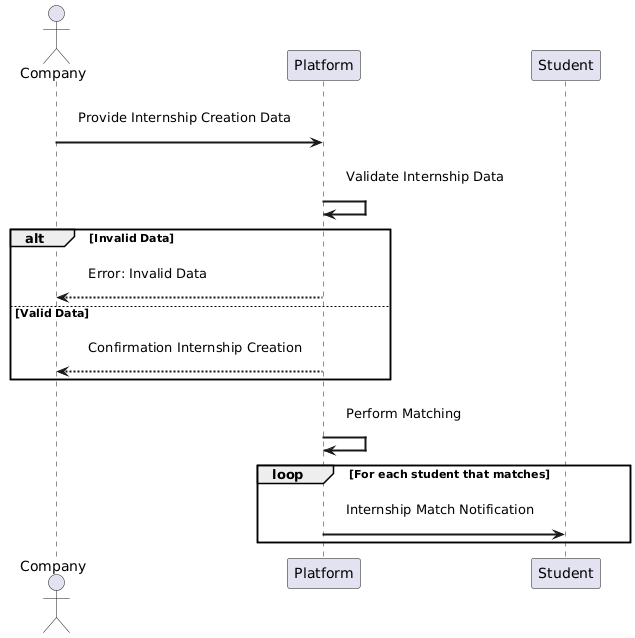
\includegraphics[scale = 0.8]{Images/ImagesRASD/Internship_post_creation_use_case.png}
\end{center}

\newpage
\textbf{4) Student updates his personal data and CV upload use case}\\

\begin{table}[h!]
    \centering
    \begin{tabular}{lp{10cm}}
        \textbf{Actor} & Student \\ \hline
        \textbf{Entry conditions} & The student is correctly logged on the S\&C platform and he is ready to submit personal data and optionally upload his CV. \\ \hline
        \textbf{Event Flow} &
        1. The student submits their skills, interests, and other personal data. \\
        & 2a. If the personal data is invalid, the platform returns an error: "Error in personal data provided." \\
        & 2b. If the personal data is valid, the platform confirms that the data was successfully uploaded. \\
        & 3. The student optionally uploads their CV. \\
        & 4a. If the CV is invalid, the platform returns an error: "Error in the file uploaded." \\
        & 4b. If the CV is valid, the platform confirms that the upload was successful. \\
        & 5. The platform performs matching based on the student data. \\
        & 6. For each matching company, the platform sends a notification about the student. \\
        \hline
        \textbf{Exit condition} & The student's personal data and, if applicable, CV are successfully uploaded and relevant companies are notified. \\ \hline
        \textbf{Exceptions} &
        2. Invalid personal data: The student must correct and resubmit their personal data. \\
        & 4. Invalid CV: The student has uploaded an invalid file. \\
    \end{tabular}
    \caption{Student updates his personal data and CV upload use case}
    \label{tab:student_data_cv_upload}
\end{table}



\begin{center}
    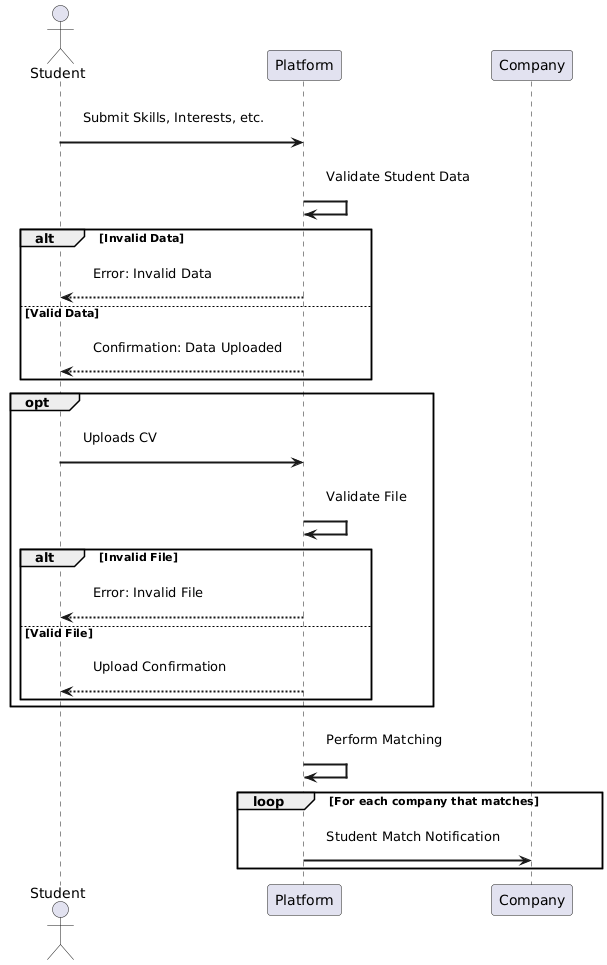
\includegraphics[scale = 0.7]{Images/ImagesRASD/Personal_data_and_CV_upload.png}
\end{center}

\newpage
\textbf{5) Student submits an application to an internship}\\

\begin{table}[h!]
    \centering
    \begin{tabular}{lp{10cm}}
        \textbf{Actor} & Student \\ \hline
        \textbf{Entry conditions} & The student is logged on the S\&C platform and he is ready to apply for an internship. The student has already updated his profile, inserting a CV and his skills and interests.\\ \hline
        \textbf{Event Flow} &
        1. The student requests a list of internships. \\
        & 2. The platform provides the list of available internships. \\
        & 3. The student selects an internship from the list. \\
        & 4. The platform provides the details of the selected internship. \\
        & 5. The student submits their application data for the selected internship. \\
        & 6. The platform validates the application data. \\
        & 7a. If the data is valid, the platform confirms that the application submission was successful. \\
        & 7b. If the data is not valid, the platform returns an error message. \\
        \hline
        \textbf{Exit condition} & The student's application for the internship is successfully submitted. \\ \hline
        \textbf{Exceptions} &
        7b. Invalid application data. \\
    \end{tabular}
    \caption{ Student submits an application to an internship}
    \label{tab:internship_application}
\end{table}


\begin{center}
    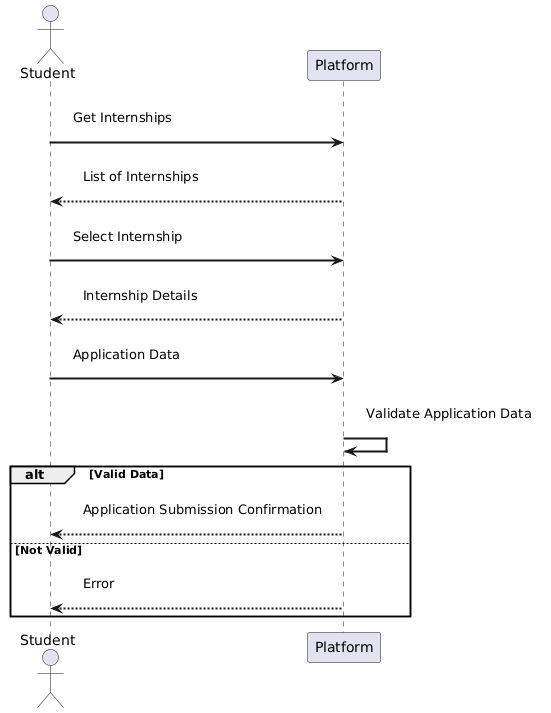
\includegraphics[scale = 0.8]{Images/ImagesRASD/Student_application.png}
\end{center}

\newpage
\textbf{6) Company manages income applications}\\

\begin{table}[h!]
    \centering
    \begin{tabular}{lp{10cm}}
        \textbf{Actor} & Company \\ \hline
        \textbf{Entry conditions} & The company is logged on the S\&C platform, ready to manage internship applications. \\ \hline
        \textbf{Event Flow} &
        1. The company requests the list of internship posts. \\
        & 2. The platform provides the list of posted internships. \\
        & 3. The company selects a specific internship from the list. \\
        & 4. The platform provides the details of the selected internship. \\
        & 5. The company requests the list of applicants for the internship. \\
        & 6. The platform provides the list of applicants. \\
        & 7. For each applicant: \\
        & \quad a. The company requests applicant information. \\
        & \quad b. The platform provides the applicant information. \\
        & \quad c. The company reviews the selected application. \\
        & \quad d. The company submits the updated application status. \\
        & \quad e. The platform updates the application status \\
        & \quad f. Application status updated successfully \\
        & \quad g. The platform sends the result to the student. \\
        \hline
        \textbf{Exit condition} & The company's review and status update for each applicant are completed, and results are sent to students. \\ \hline
        \textbf{Exceptions} & None specified. \\
    \end{tabular}
    \caption{Company management of internship applications use case}
    \label{tab:company_manage_internship_applications}
\end{table}


\begin{center}
    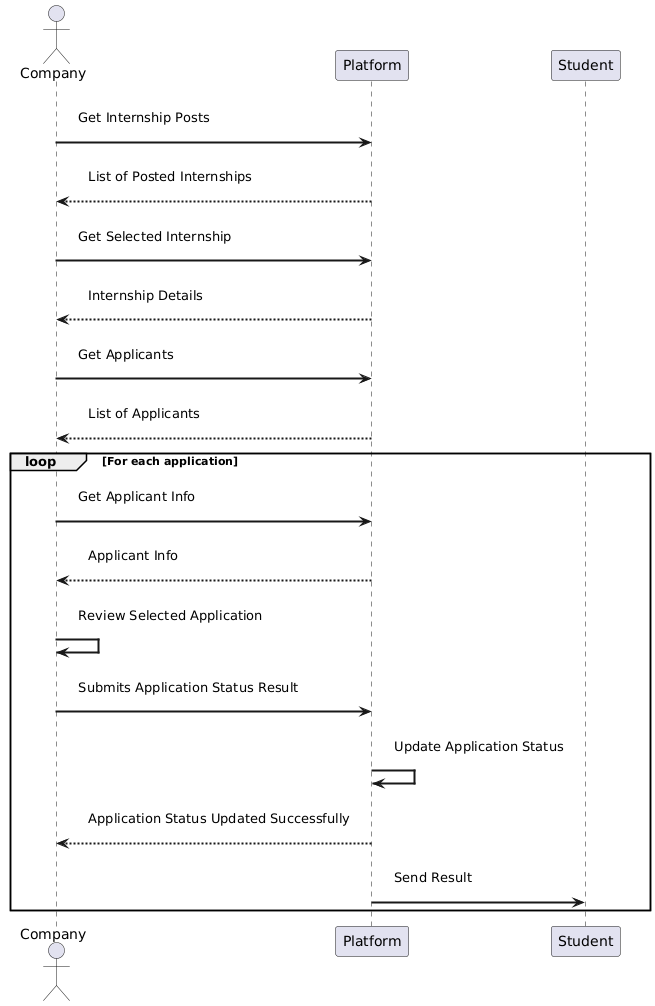
\includegraphics[scale = 0.7]{Images/ImagesRASD/Company_to_manage_income_applications.png}
\end{center}

\newpage
\textbf{7) Student sends online assessment answers}\\

\begin{table}[h!]
    \centering
    \begin{tabular}{lp{10cm}}
        \textbf{Actor} & Student \\ \hline
        \textbf{Entry conditions} & The student is loggede on the platform, has passed the screening of the specific application and ready to respond to the online assessment questions. The student is already on the appropriate online assessment page on the platform.  \\ \hline
        \textbf{Event Flow} &
        1. The student responds to each question individually. \\
        & 2. After answering all questions, the student sends their answers to the platform. \\
        & 3. The platform validates the submitted answers. \\
        & 4a. If the answers are valid, the platform saves the answers and sends a confirmation to the student. \\
        & 4b. If the answers are not valid, the platform sends an error message to the student indicating that revision is needed. \\
        \hline
        \textbf{Exit condition} & The student's answers are successfully validated and saved on the platform, or the student is notified to revise the answers. \\ \hline
        \textbf{Exceptions} &
        4. Invalid answers: The student must revise their answers. \\
    \end{tabular}
    \caption{Student answer submission and validation use case}
    \label{tab:student_answer_submission}
\end{table}


\begin{center}
    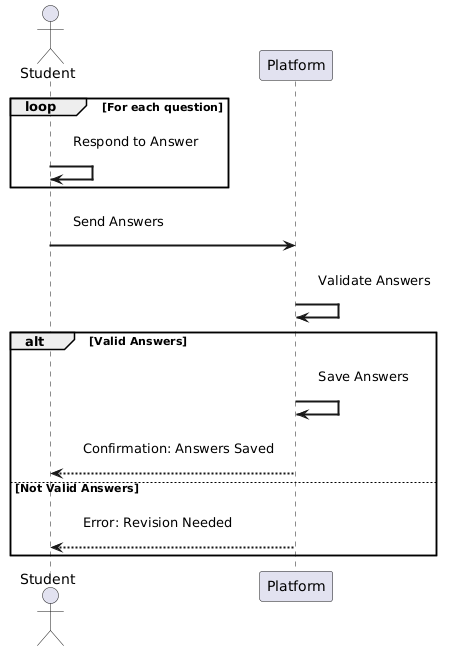
\includegraphics[scale = 0.8]{Images/ImagesRASD/Student_sending_answers.png}
\end{center}

\newpage
\textbf{8) Company reviews online assessment questions}\\

\begin{table}[h!]
    \centering
    \begin{tabular}{lp{10cm}}
        \textbf{Actor} & Company \\ \hline
        \textbf{Entry conditions} & The company is logged on the platform and it is ready to manage one of its internship online assessment questions. \\ \hline
        \textbf{Event Flow} &
        1. The company requests the list of internship posts. \\
        & 2. The platform provides the list of posted internships. \\
        & 3. The company selects a specific internship from the list. \\
        & 4. The platform provides the details of the selected internship. \\
        & 5. The company requests the list of applicants for the internship. \\
        & 6. The platform provides the list of applicants. \\
        & 7. For each applicant that has answered the questions: \\
        & \quad a. The company requests the applicant's answers. \\
        & \quad b. The platform provides the applicant's answers. \\
        & \quad c. The company reviews the applicant's answers. \\
        & \quad d. The company submits the application status result. \\
        & \quad e. The platform updates the application status result \\
        & \quad f. The platform confirms to the company the successful update of the application status. \\
        & \quad g. The platform sends the result to the student. \\
        \hline
        \textbf{Exit condition} & The company's review and status update for each applicant are completed, and results are sent to the students. \\ \hline
        \textbf{Exceptions} & None specified. \\
    \end{tabular}
    \caption{Company management of internship applications use case}
    \label{tab:company_manage_internship_applications}
\end{table}

\begin{center}
    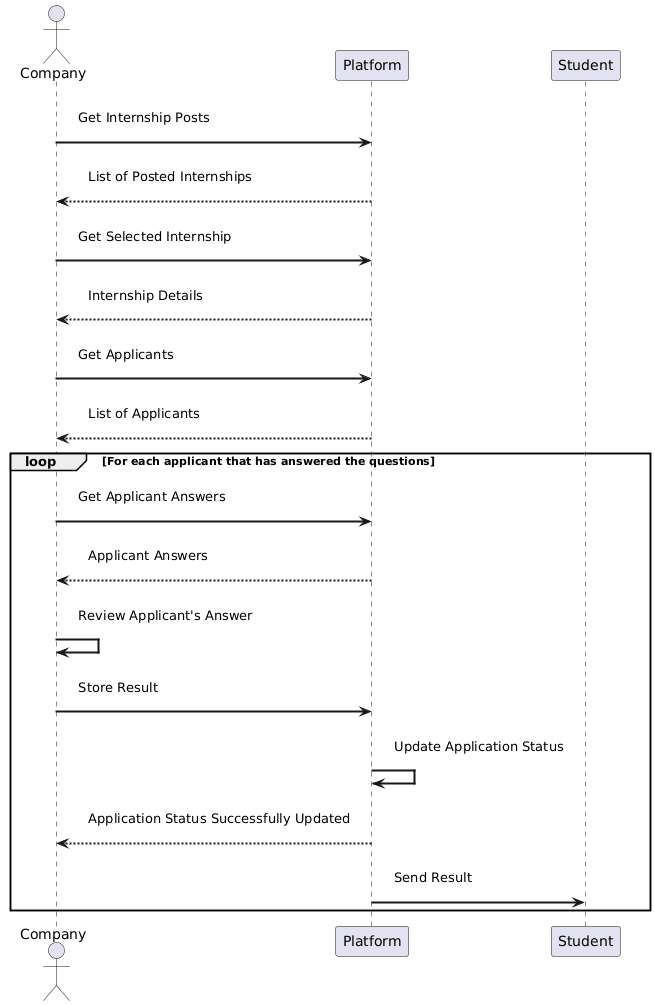
\includegraphics[scale = 0.70]{Images/ImagesRASD/Company_questions_reviewing.png}
\end{center}
\newpage

\textbf{9) Student or Company sends a feedback about the internship}\\

\begin{table}[h!]
    \centering
    \begin{tabular}{lp{10cm}}
        \textbf{Actor} & Student or Company \\ \hline
        \textbf{Entry conditions} & The student or the company provides a feedback on his experience with the internship. The actor is effectively involved in the related internship.\\ \hline
        \textbf{Event Flow} &
        1. The actor selects the internship to review. \\
        & 2. The platform responds with the internship details. \\
        & 3. The actor sends the feedback. \\
        & 4. The platform validates the provided feedback \\
        & 5a. The platform responds with a confirmation feedback in case the validation is successful. \\
        & 5b. The platform responds with an error feedback in case the validation has not been successful . \\
        \hline \textbf{Exit condition} & The feedback is well completed, and registered.\\
        \hline \textbf{Exceptions} & The validation of the feedback has been not successful. \\ \end{tabular}
    \caption{ Student or Company sends a feedback about the internship}
    \label{tab:company_manage_internship_applications}
\end{table}

\begin{center}
    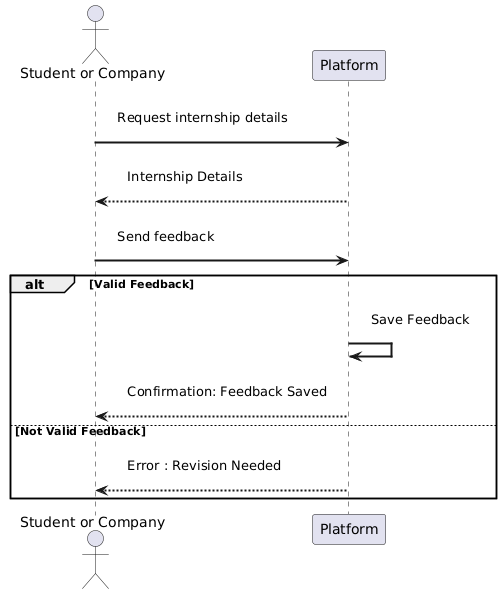
\includegraphics[scale = 0.8]{Images/ImagesRASD/StudentAndCompanySendFeedback.png}
\end{center}
\newpage

\textbf{10) Student or Company sends a feedback about the platform} \\

\begin{table}[h!]
    \centering
    \begin{tabular}{lp{10cm}}
        \textbf{Actor} & Student or Company \\ \hline
        \textbf{Entry conditions} & The student or the company provides a feedback on his experience on the platform.\\ \hline
        \textbf{Event Flow} &
        1. The actor sends a platform feedback. \\
        & 2. The platform validates the provided feedback \\
        & 3a. The platform responds with a confirmation feedback in case the validation is successful. \\
        & 3b. The platform responds with an error feedback in case the validation has not been successful . \\
        \hline \textbf{Exit condition} & The feedback is well completed, and has been correctly registered.\\
        \hline \textbf{Exceptions} & The feedback provided is not valid. \\ \end{tabular}
    \caption{The student or the company provides a feedback on his experience on the platform.}
    \label{tab:company_manage_internship_applications}
\end{table}

\begin{center}
    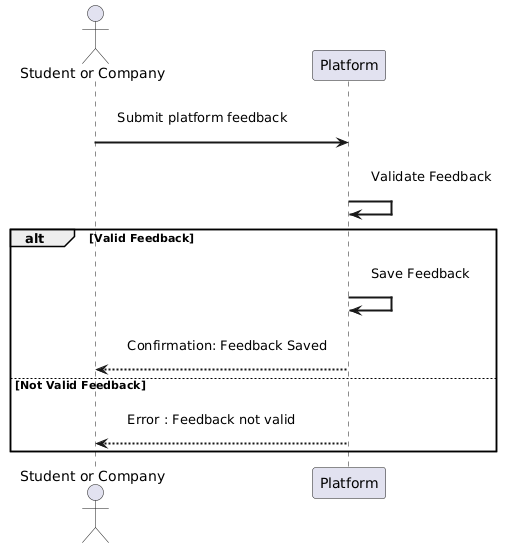
\includegraphics[scale = 0.8]{Images/ImagesRASD/StudentAndCompanySendPlatformFeedback.png}
\end{center}
\newpage

\textbf{11) University monitors the progress of internships}\\

\begin{table}[h!]
    \centering
    \begin{tabular}{lp{10cm}}
        \textbf{Actor} & University \\ \hline
        \textbf{Entry conditions} & The university is correctly logged on the plaform and he is ready to monitor an internship. \\ \hline
        \textbf{Event Flow} &
        1. The university requests a list of internships  from the platform. \\
        & 2. The platform returns the list of internships(including only those which involve students of that university). \\
        & 3. The university selects a specific internship. \\
        & 4. The platform returns the internship details. \\
        & 5. The university reviews the internship. \\
        & 6. The university optionally performs a monitoring action. \\
        & 7a. The platform confirms that the action has been successfully applied. \\
        & 7b. The platform returns an error, since the action is not valid. \\
        \hline
        \textbf{Exit condition} & Monitoring results (success or error) are retrieved, and relevant information is displayed or stored. \\ \hline
        \textbf{Exceptions} & Missing data for monitoring action.
    \end{tabular}
    \caption{University monitors the progress of internships}
    \label{tab:university_monitors_internships}
\end{table}


\begin{center}
    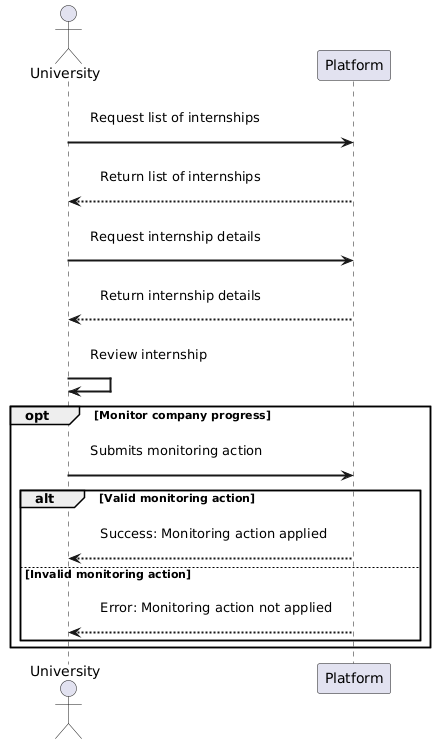
\includegraphics[scale = 0.8]{Images/ImagesRASD/University_check_status.png}
\end{center}
\newpage

\subsection{Summary of the Functional Requirements}
\begin{longtable}{|p{0.1\textwidth}|p{0.9\textwidth}|}
    \hline

    \textbf{R1} & The S\&C shall allow users to log in to their accounts using their registered email and password. \\
    \hline
    \textbf{R2} & The S\&C shall allow users to reset their password via a “Forgot Password” feature, with verification sent to their registered email. \\
    \hline
    \textbf{R3} & The S\&C shall allow users to log out securely from their accounts. \\
    \hline
    \textbf{R4} & The S\&C shall allow users to register on the platform. \\
    \hline

    \textbf{R5} & The S\&C shall allow students to edit profiles and upload CV. \\
    \hline
    \textbf{R6} & The S\&C shall allow students to edit personal details, skills, and interests in their profiles. \\
    \hline
    \textbf{R7} & The S\&C shall allow students to submit assessments, including answering open-ended and multiple-choice questions. \\
    \hline

    \textbf{R8} & The S\&C shall provide students with an internship search tool that includes filtering options for location, field of study, and publication date. \\
    \hline
    \textbf{R9} & The S\&C shall allow students to get tailored internship suggestions based on their interests. \\
    \hline
    \textbf{R10} & The S\&C shall allow the recommendation engine to improve over time based on feedback from students and companies. \\
    \hline

    \textbf{R12} & The S\&C shall allow real-time tracking of application statuses, showing students the progress of applications at each stage. \\
    \hline
    \textbf{R13} & The S\&C shall allow companies to view submitted applications. \\
    \hline
    \textbf{R14} & The S\&C shall allow companies to accept or reject candidates directly from the submitted applications. \\
    \hline

    \textbf{R15} & The S\&C shall allow companies to create internship postings, specifying job roles and required skills. \\
    \hline
    \textbf{R16} & The S\&C shall allow companies to edit existing internship postings after creation. \\
    \hline

    \textbf{R17} & The S\&C shall allow companies to have a dashboard to review candidate applications and filter profiles. \\
    \hline
    \textbf{R18} & The S\&C shall allow companies access to a comprehensive page to track applications status. \\
    \hline
    \textbf{R19} & The S\&C shall allow companies to have a recommendation feed for candidates based on internship requirements. \\
    \hline
    \textbf{R20} & The S\&C shall allow companies to access a "Potential Candidates" feature to view potential matches based on student profiles. \\
    \hline

    \textbf{R21} & The S\&C shall allow both students and companies to provide feedback, covering overall satisfaction. \\
    \hline
    \textbf{R22} & The S\&C shall allow companies to view feedback provided for candidates from previous internships. \\
    \hline
    \textbf{R23} & The S\&C shall allow students to view feedback provided for companies from previous interns. \\
    \hline

    \textbf{R24} & The S\&C shall allow universities to monitor feedback scores to ensure professional standards are met during internships. \\
    \hline
    \textbf{R25} & The S\&C shall allow a reporting feature for users to report inappropriate or irrelevant internship environments, ensuring a safe and professional place. \\
    \hline
    \textbf{R26} & The S\&C shall allow universities to write feedback on the platform to suggest improvements. \\
    \hline
    \textbf{R27} & The S\&C shall allow universities to write feedback directly to students and companies. \\
    \hline
    \textbf{R28} & The S\&C shall allow suggestions to students on what skills to achieve based on their interests. \\
    \hline
    \textbf{R29} & The S\&C shall allow the platform to provide suggestions to companies for improving the quality and clarity of their internship descriptions. \\
    \hline



\end{longtable}
\newpage
\subsection{Mapping on Goals}
In the following table it is shown how the different goals map on the requirements and domain assumptions described in the previous chapters. Furthermore, the mapping is made in order to make this formula hold
\begin{equation}
    R \land D \models G
\end{equation}
\begin{longtable}{| p{0.3\textwidth} | p{0.4\textwidth} | p{0.3\textwidth} |}
    \hline
    \textbf{Goal} & \textbf{Domain Assumptions (DA)} & \textbf{Requirements (R)} \\
    \hline
    G1: Students can search for internships that match their skills and career goals. & DA1: Students have varied skills and interests. \newline DA8: Students are enrolled in the university they selected. & R5: Allow students to create/edit profiles, upload CVs, and validate them in real-time. \newline R6: Allow students to edit personal details, skills, and interests in their profiles. \newline R8: Provide a search tool with filtering options for location, field of study, and publication date. \\ \hline

    G2: Companies can advertise internships and engage suitable candidates. & DA2: Companies have specific internship requirements. \newline DA9: The company account accurately corresponds to the respective company. & R15: Allow companies to create internship postings, specifying job roles and required skills. \newline R16: Allow companies to edit existing internship postings after creation. \newline R17: Provide companies with a dashboard to review candidate applications and filter profiles. \\ \hline

    G3: The platform can recommend relevant internships to students. & DA1: Students have varied skills and interests. \newline DA8: Students are enrolled in the university they selected. & R5: Allow students to create/edit profiles, upload CVs, and validate them in real-time. \newline R6: Allow students to edit personal details, skills, and interests in their profiles. \newline R9: Provide tailored internship suggestions based on students' interests. \newline R10: Improve the recommendation engine over time using feedback from students and companies. \newline R28: Suggest skills for students to develop based on their interests. \\ \hline

    G4: The platform can recommend potential candidates to companies. & DA2: Companies have specific internship requirements. \newline DA9: The company account accurately corresponds to the respective company. & R15: Allow companies to create internship postings, specifying job roles and required skills. \newline R17: Provide companies with a dashboard to review candidate applications and filter profiles. \newline R19: Provide companies with a recommendation feed for candidates based on internship requirements. \newline R20: Enable companies to view potential matches through a "Potential Candidates" feature. \\ \hline

    G5: Companies can manage the selection process through an interview management system. & DA2: Companies have specific internship requirements. \newline DA9: The company account accurately corresponds to the respective company. & R13: Allow companies to view submitted applications. \newline R14: Allow companies to accept or reject candidates directly from submitted applications. \newline R17: Provide companies with a dashboard to review candidate applications and filter profiles. \newline R18: Enable companies to track application statuses through a comprehensive page. \\ \hline

    G6: Companies can evaluate candidates. & DA2: Companies have specific internship requirements. \newline DA9: The company account accurately corresponds to the respective company. & R13: Allow companies to view submitted applications. \newline R14: Allow companies to accept or reject candidates directly from submitted applications. \newline R22: Enable companies to view feedback provided for candidates from previous internships. \\ \hline

    G7: Students and companies can provide feedback to continuously improve the matchmaking process. & DA1: Students have varied skills and interests. \newline DA2: Companies have specific internship requirements. & R21: Allow both students and companies to provide feedback covering overall satisfaction. \newline R22: Enable companies to view feedback provided for candidates from previous internships. \newline R23: Allow students to view feedback provided for companies from previous interns. \newline R25: Provide a reporting feature for users to report inappropriate or irrelevant internship environments. \\ \hline

    G8: Universities can track and assess the ongoing progress of internships. & DA7: The student and the university successfully register as a student and university, respectively. & R24: Allow universities to monitor feedback scores to ensure professional standards. \newline R26: Enable universities to provide feedback on the platform to suggest improvements. \newline R27: Allow universities to provide feedback directly to students and companies. \\ \hline

    G9: The platform can provide suggestions to improve CVs. & DA1: Students have varied skills and interests. \newline DA3: The students need to provide a valid email address. & R5: Allow students to create/edit profiles, upload CVs, and validate them in real-time. \newline R6: Allow students to edit personal details, skills, and interests in their profiles. \newline R28: Suggest skills for students to develop based on their interests. \\ \hline

    G10: The platform can provide suggestions to companies to improve internship description. & DA2: Companies have specific internship requirements. \newline DA4: The companies need to provide a valid email. & R15: Allow companies to create internship postings, specifying job roles and required skills. \newline R16: Allow companies to edit existing internship postings after creation. \newline R29: Suggest improvements to companies for the quality and clarity of their internship descriptions. \\ \hline

\end{longtable}


\begin{itemize}
    \item \textbf{Student Profile Management}:
    \begin{itemize}
        \item Students can create and manage profiles, including personal details, education history, skills, and work experience.
        \item The profile interface will support dynamic updates, and validation of critical fields to ensure profile completeness.
        \item Uploaded CVs must be in PDF or DOCX format, and the system must validate that the upload meets the required format.
        \item Profiles must support a review system where students can preview how their information will appear to potential employers.
    \end{itemize}
    \item \textbf{Internship Listings}:
    \begin{itemize}
        \item Companies can create, update, and delete internship listings with detailed descriptions, requirements, and benefits.
        \item Listings must include filters for location, skills, and compensation, allowing students to search effectively.
        \item The system must allow companies to specify internship deadlines, and automatically remove expired listings.
        \item A dynamic feedback mechanism will notify companies about the completeness and attractiveness of their internship postings, suggesting improvements if needed.
    \end{itemize}
    \item \textbf{Recommendation System}:
    \begin{itemize}
        \item The recommendation engine must take into account factors such as the student’s skills, location preferences, previous internships, and company requirements.
        \item The engine will learn and improve over time using feedback data from previous internships, adjusting future recommendations based on the outcomes and feedback provided by both students and companies.
    \end{itemize}
    \item \textbf{Selection and Interview Process}:
    \begin{itemize}
        \item Companies can select candidates for interviews and manage interview schedules directly through the platform.
        \item Structured questionnaires will be provided by companies for student applicants to complete prior to interviews, with results stored in the system for company review.
        \item Companies will be able to log interview outcomes, including scores and qualitative feedback, directly into the system to aid decision-making.
    \end{itemize}
    \item \textbf{Feedback Collection}:
    \begin{itemize}
        \item After each internship, both students and companies must provide structured feedback on the experience.
        \item The feedback must cover multiple dimensions, including skills demonstrated, professionalism, and overall satisfaction.
        \item The system will anonymize feedback to comply with GDPR regulations, ensuring privacy for both parties involved.
        \item The feedback will be used as a data source for improving the recommendation system and internship matching algorithm.
    \end{itemize}
    \item \textbf{Complaint Handling}:
    \begin{itemize}
        \item Universities must have access to a complaint management system, allowing them to view and manage complaints filed by either students or companies.
        \item Complaints must be classified by type (e.g., harassment, contract breach) and tracked through a resolution workflow.
        \item Complaints can be escalated for review by a university administrator, who will have access to the full history of the issue.
        \item The system will automatically notify all relevant parties (students, companies, administrators) of complaint status updates.
    \end{itemize}
\end{itemize}

\section{Performance Requirements}

\subsection{Number of Users}
The platform will be used by multiple parties, including students, companies, and universities. Based on market research, which includes a comparison with existing similar platforms such as the CareerService platform for Politecnico di Milano (Polimi) and other internship-matching services across Europe, we estimate that S\&C will attract approximately 20,000 students and 2,500 companies from various universities and industries. Additionally, around 50 universities will be actively using the platform to monitor internships. This gives us an estimated total user base of 22,550 users.\\ \\
Considering a worst-case scenario where 40\% of the users are active simultaneously, the system must support up to 9,020 concurrent users. The platform must ensure smooth operation, even during peak usage times.

\subsection{Data Storage}
The platform needs to store various types of data related to students, companies, internships, and the matchmaking process. Below are the estimated storage requirements for the first year of operation:

\begin{itemize}
    \item \textbf{Student data (profile)}: Each student will have a profile containing personal information such as name, contact details, and skillset. This profile data is estimated to require around 10 KB per student. Considering 20,000 students:
    \[
        20,000 \times 10 \, \text{KB} = 195.3 \, \text{MB}
    \]

    \item \textbf{Student data (PDF CVs)}: In addition to the basic profile information, each student is expected to upload their CV in PDF format. The average size of a CV in PDF format is estimated to be around 300 KB. Thus, for 20,000 students:
    \[
        20,000 \times 300 \, \text{KB} = 5.72 \, \text{GB}
    \]

    \item \textbf{Company data}: Each company will have a profile including company information, project descriptions, and internship offerings. Assuming 15 KB of storage per company profile and considering 2,500 companies:
    \[
        2,500 \times 15 \, \text{KB} = 36.6 \, \text{MB}
    \]

    \item \textbf{Internship postings}: Each internship posting will include information about the project, tasks, technologies, and terms (e.g., paid/unpaid). Assuming each posting requires 10 KB and that each company posts five internships a year:
    \[
        2,500 \times 5 \times 10 \, \text{KB} = 122.1 \, \text{MB}
    \]

    \item \textbf{Student feedback and internship outcomes}: Feedback data provided by students and companies will be stored for analysis. Assuming 5 KB per feedback submission and expecting each internship to receive three feedback entries, for 10,000 matched internships in the first year:
    \[
        10,000 \times 3 \times 5 \, \text{KB} = 146.5 \, \text{MB}
    \]

    \item \textbf{Interview and selection data}: Information about interviews, questionnaires, and selection processes will also be stored. Assuming 8 KB per interview record and that each company interviews an average of five candidates per internship:
    \[
        10,000 \times 5 \times 8 \, \text{KB} = 390.6 \, \text{MB}
    \]
\end{itemize}

Summing all storage requirements for the first year:
\[
    195.3 \, \text{MB} + 5.72 \, \text{GB} + 36.6 \, \text{MB} + 122.1 \, \text{MB} + 146.5 \, \text{MB} + 390.6 \, \text{MB} = 6.6 \, \text{GB}
\]\\
Thus, a storage allocation of \textbf{10 GB} will be sufficient to accommodate the platform's data storage needs for a year, including room for growth and additional data generated by the system.


\subsection{Time Response}
Although there are no strict time requirements for the S\&C platform, it is important to maintain a responsive user experience. Reasonable average response times for key interactions could be as follows:
\begin{itemize}
    \item Basic search queries and browsing operations should ideally be processed within \textbf{2 seconds}, to ensure a smooth navigation experience.
    \item More complex operations, such as generating personalized internship recommendations, should aim to complete within \textbf{5 seconds}, balancing the computational effort required with acceptable wait times for the user.
\end{itemize}

\section{Design Constraints}

\subsection{Standards Compliance}

The platform must adhere to EU's GDPR regulations to ensure secure data storage and transmission, particularly when handling sensitive student and company data. All data interactions must comply with GDPR provisions regarding data ownership, user consent, and the right to access and delete data.

Additionally, the platform must comply with industry security standards to ensure the system is secure against potential threats.

\subsection{Hardware Limitations}

There are no specific hardware limitations imposed on end-users.

\section{Software System Attributes}

\subsection{Reliability}
The S\&C platform must be reliable to ensure continuous operation, even in the presence of faults. The system should be designed to be fault-tolerant to prevent the propagation of errors and ensure uninterrupted usability. Mechanisms such as automated failover and data redundancy should be in place to mitigate the risk of downtime due to unexpected failures.

\subsection{Availability}
The platform must be available as much as possible, with a minimum uptime of 99.999\%. Scheduled maintenance breaks should be minimized and, when necessary, performed during low-traffic periods (e.g., nighttime) to avoid disrupting critical usage, particularly around high-demand periods such as internship application deadlines.

\subsection{Security}
Security is critical for the S\&C platform, as it handles sensitive student and company data. The system must implement strong authentication and authorization mechanisms. Authentication should ensure that users are properly identified before accessing the platform, while authorization should ensure that users can only perform actions they are permitted to.

\subsection{Maintainability}
The platform should be designed with scalability and modularity in mind to facilitate the easy addition of new features or modifications with minimal effort. The use of reusable code components and modular architecture will aid in making future updates efficient. Regular maintenance operations should be scheduled during times of low user activity, such as nighttime, to minimize disruptions to users.

\subsection{Portability}
The S\&C platform must be accessible from a wide range of web browsers, ensuring compatibility across all major platforms (e.g., Chrome, Firefox, Safari, and Edge). On the client side, the platform should ensure  accessibility on desktop devices. No specific portability requirements are imposed on the server side, provided the platform can run on common server configurations.


\newpage
